The results from analyses with this data will be displayed in three
plots, described below and generated automatically during processing:

\subsubsection{Score plot}
Figure \ref{fig:all} displays the raw results as a point plot per algorithm and
dataset. With a reasonably small number of datasets as we have here, the plot is
quite informative; however, as the number of datasets increases it will become
more and more dense. It describes the distribution of scores over subjects
within a single dataset and for a single algorithm.

\subsubsection{Ranking plot}
The ranking
plot is intended to be a quick way of ordering algorithms, based on
the statistical significance returned by the procedure described in
Section \ref{stats}. It describes which pipelines significantly
out-performed others across all datasets.

\subsubsection{Paired plot}
Figures \ref{fig:am} and \ref{fig:csp} show ranking plots. In order to
look at two algorithms in more detail, for particular pairs of
algorithms we also offer a plot of the score in one versus the score in the other,
for all subjects across all datasets. This is computed for all pairs
of algorithms, but for use in a publication it is cumbersome to add
all the plots.

\subsubsection{Time plot}
Figure \ref{fig:time} shows a plot of training size versus fitting
time for the model. In addition to accuracy, model fitting time can also affect which
pipeline is most appropriate for a given situation. This is a function
of the number of channels, timepoints, and samples, but a point
cloud in three-dimensions is difficult to visualize on paper. As such,
for these written reports, a plot is generated of the time versus the product of the
number of channels and the number of samples (the number of timepoints
is less important as features are usually computed over all of
them). While some of the nuance is lost, it is still easy to see how
algorithms compare to each other.

We would last like to note that the results are too complex to easily
simplify into static plots. What if one, for example, wants to know
whether a pipeline only performs well on a subset of datasets? Because
of this an interactive visualization would be strongly preferred.

Figure \ref{fig:all} shows all the results generated by this entire
processing chain. Surprisingly, perhaps, the pipelines do not clearly
cluster on the dataset level, making it unclear which ones perform
best from simply this plot. What is very clear, however, is that
different datasets have very different average scores
independent of pipeline.

Figure \ref{fig:am} shows the pairwise comparison of the log
variance-based pipeline with CSP and the tangent space SVM. What is
very clearly shown both in the plots and the statistics is that, for
within-session scoring, it is strongly out-performed by both.

Figure \ref{fig:csp} shows the pairwise comparison of 
plain CSP with the two regularized approaches and with
tangent space SVM. For both the regularized approaches. while there is
a great deal of variance across subjects, the score from CSP and the
regularized CSP roughly track each other, such that there is no
significant difference between them. The only significant difference
is with the tangent space method.

Figure \ref{fig:time} shows how all the described methods compare in
terms of processing time. Unsurprisingly, the methods based on
Riemannian computation are more computationally expensive at large
sample sizes than the other methods (due to the iterative computations
and the increase in feature number). 

\begin{figure*}
    \centering
    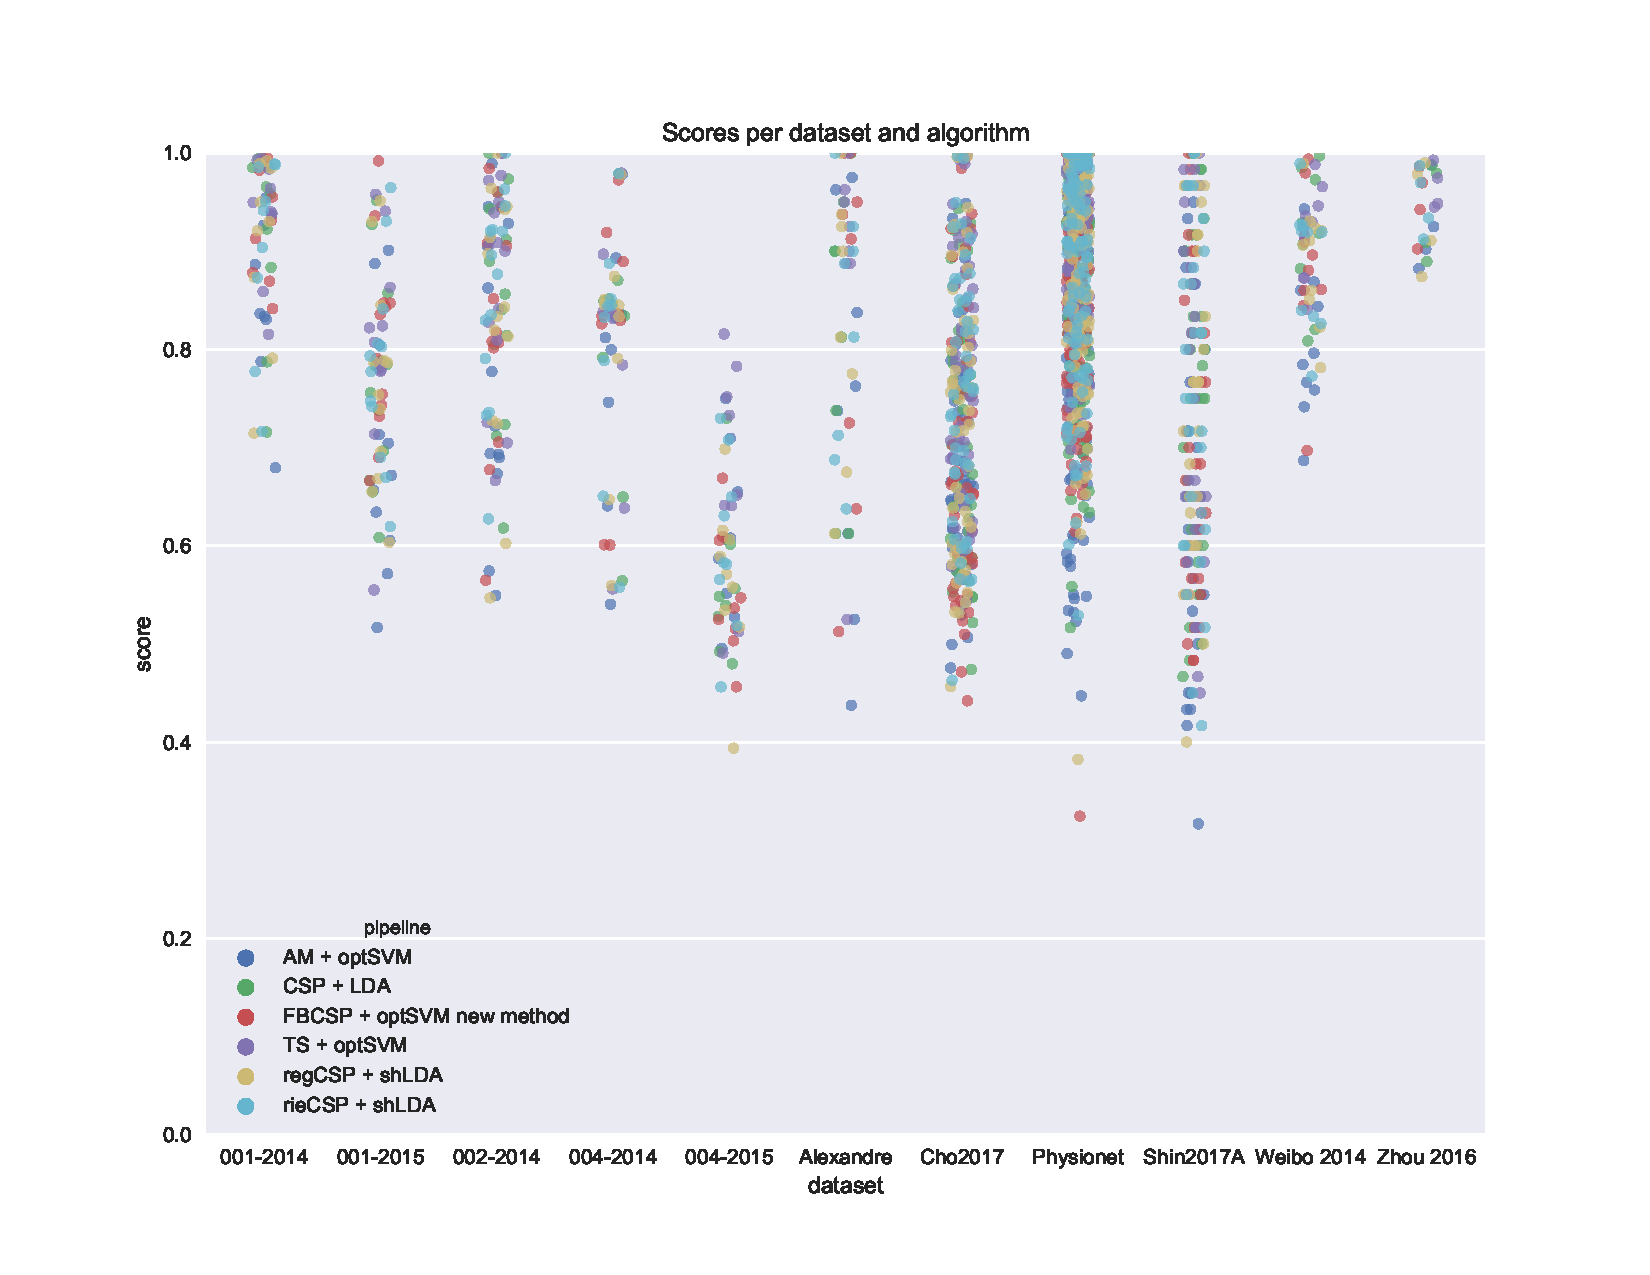
\includegraphics[width=\textwidth]{Figures/full_scores.pdf}
    \caption{Visualization of all generated scores, across all datasets.}
    \label{fig:all}
\end{figure*}
\begin{figure*}
    \centering
    \begin{subfigure}{0.5\textwidth}
        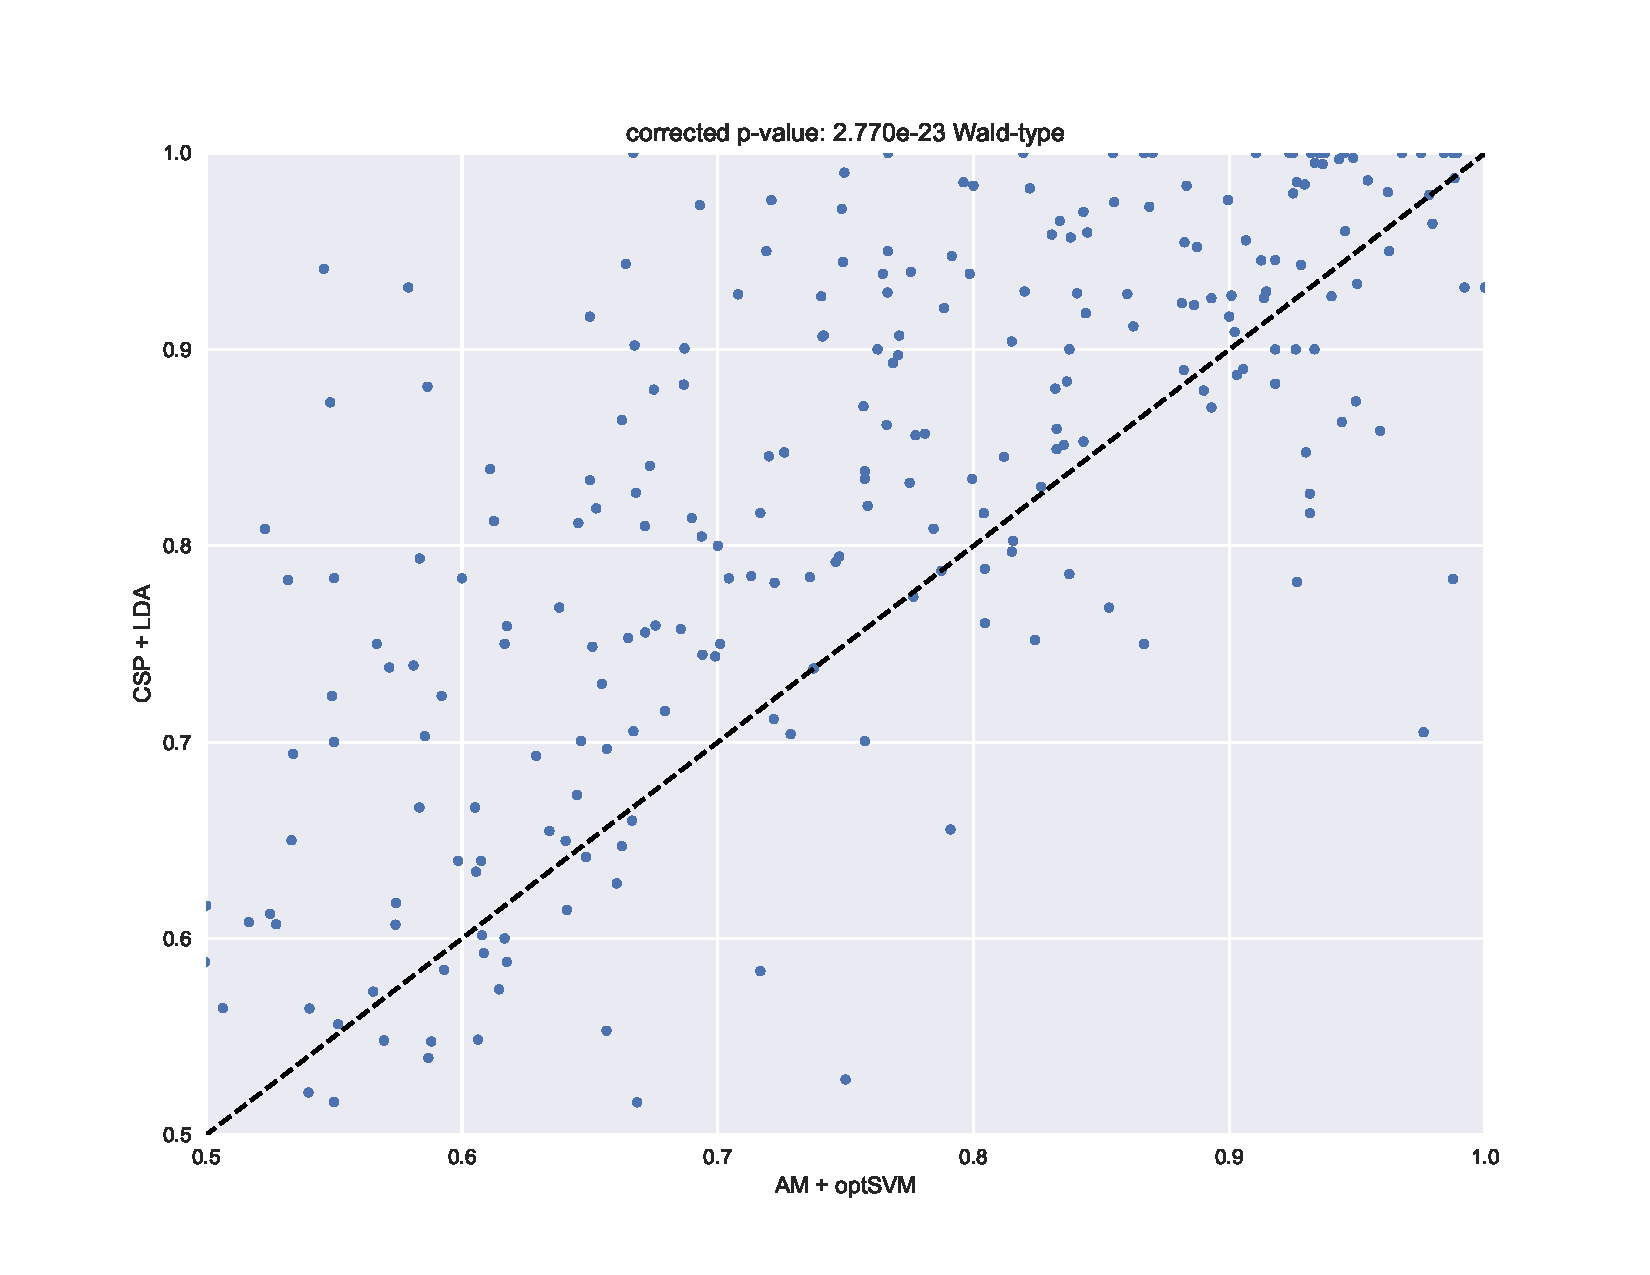
\includegraphics[width=\textwidth]{Figures/AM1.pdf}
    \end{subfigure}%
    \begin{subfigure}{0.5\textwidth}
        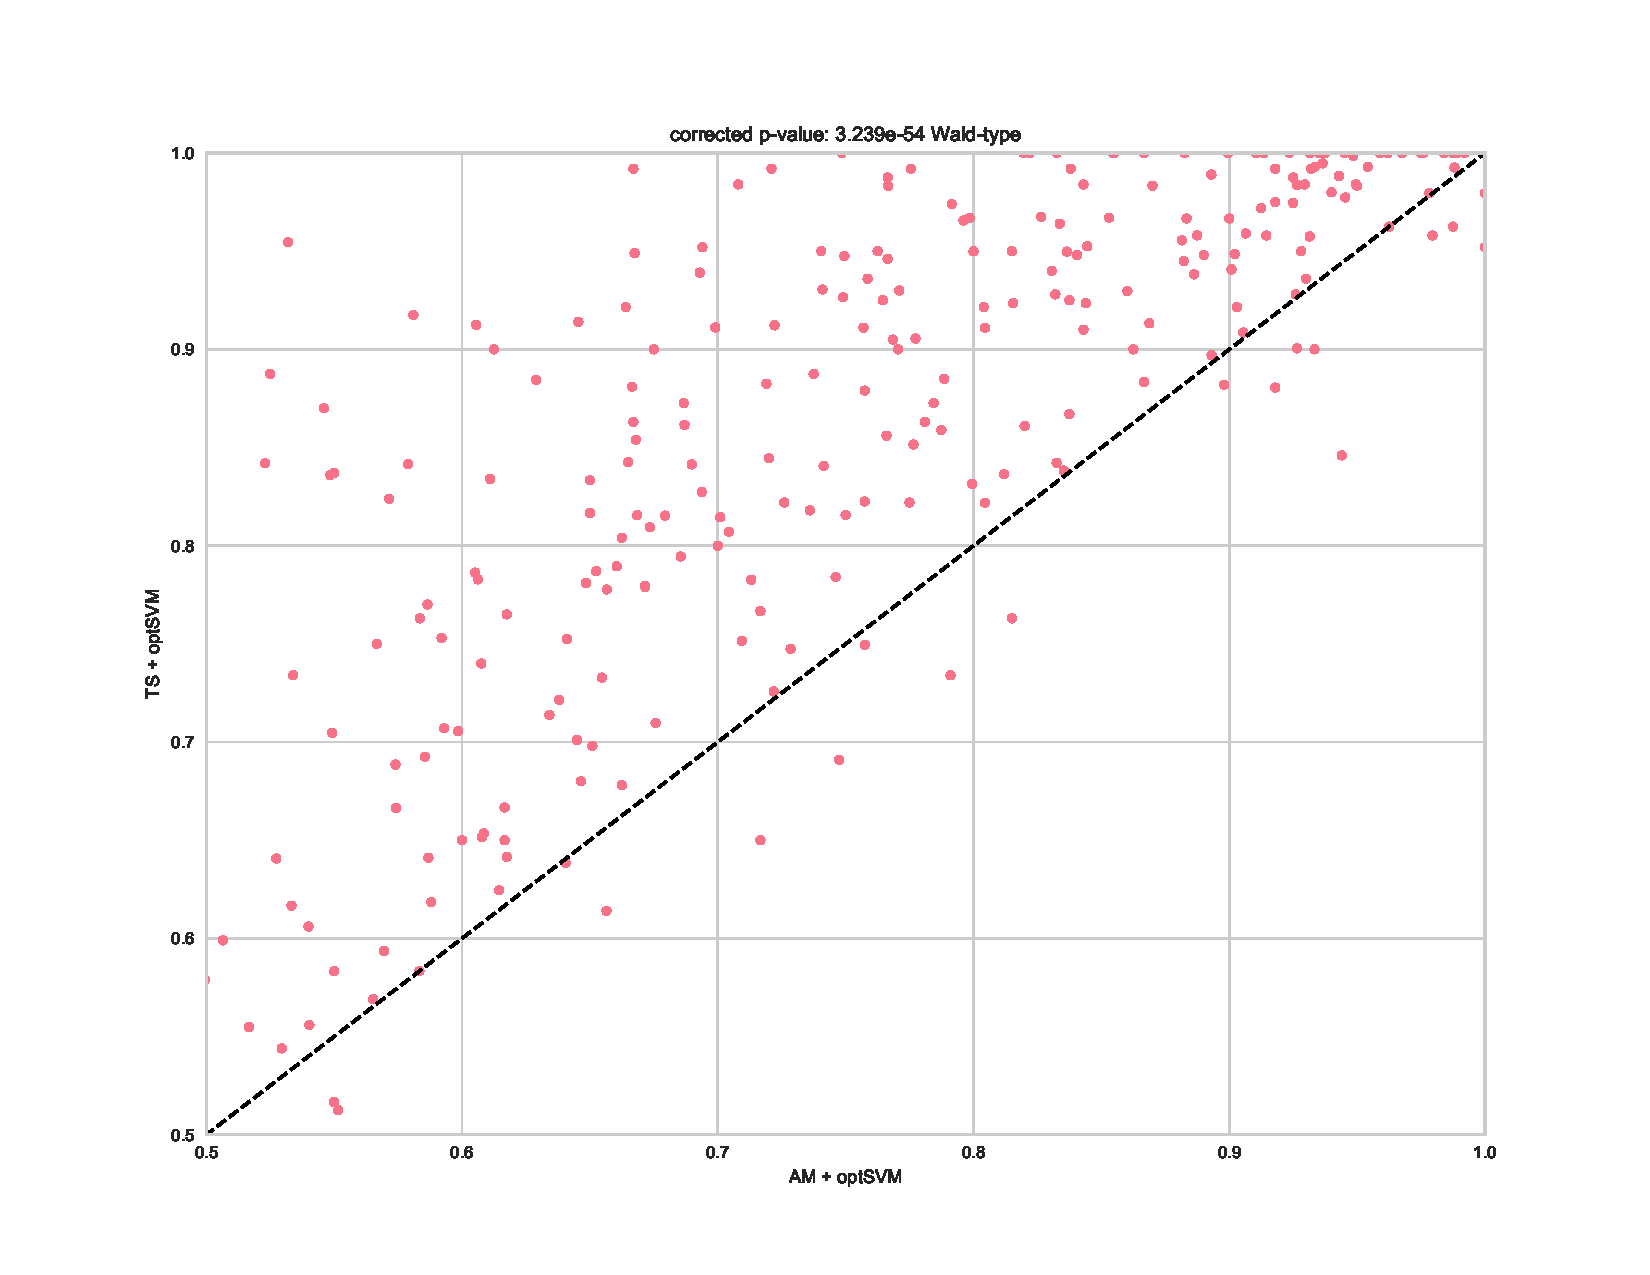
\includegraphics[width=\textwidth]{Figures/AM2.pdf}
    \end{subfigure}
    \caption{Paired plots of log variance versus basic CSP and the
      tangent space projection. It does
      consistently worse than both CSP and the tangent space method.}
    \label{fig:am}
\end{figure*}
\begin{figure*}
    \centering
    \begin{subfigure}{0.475\textwidth}
        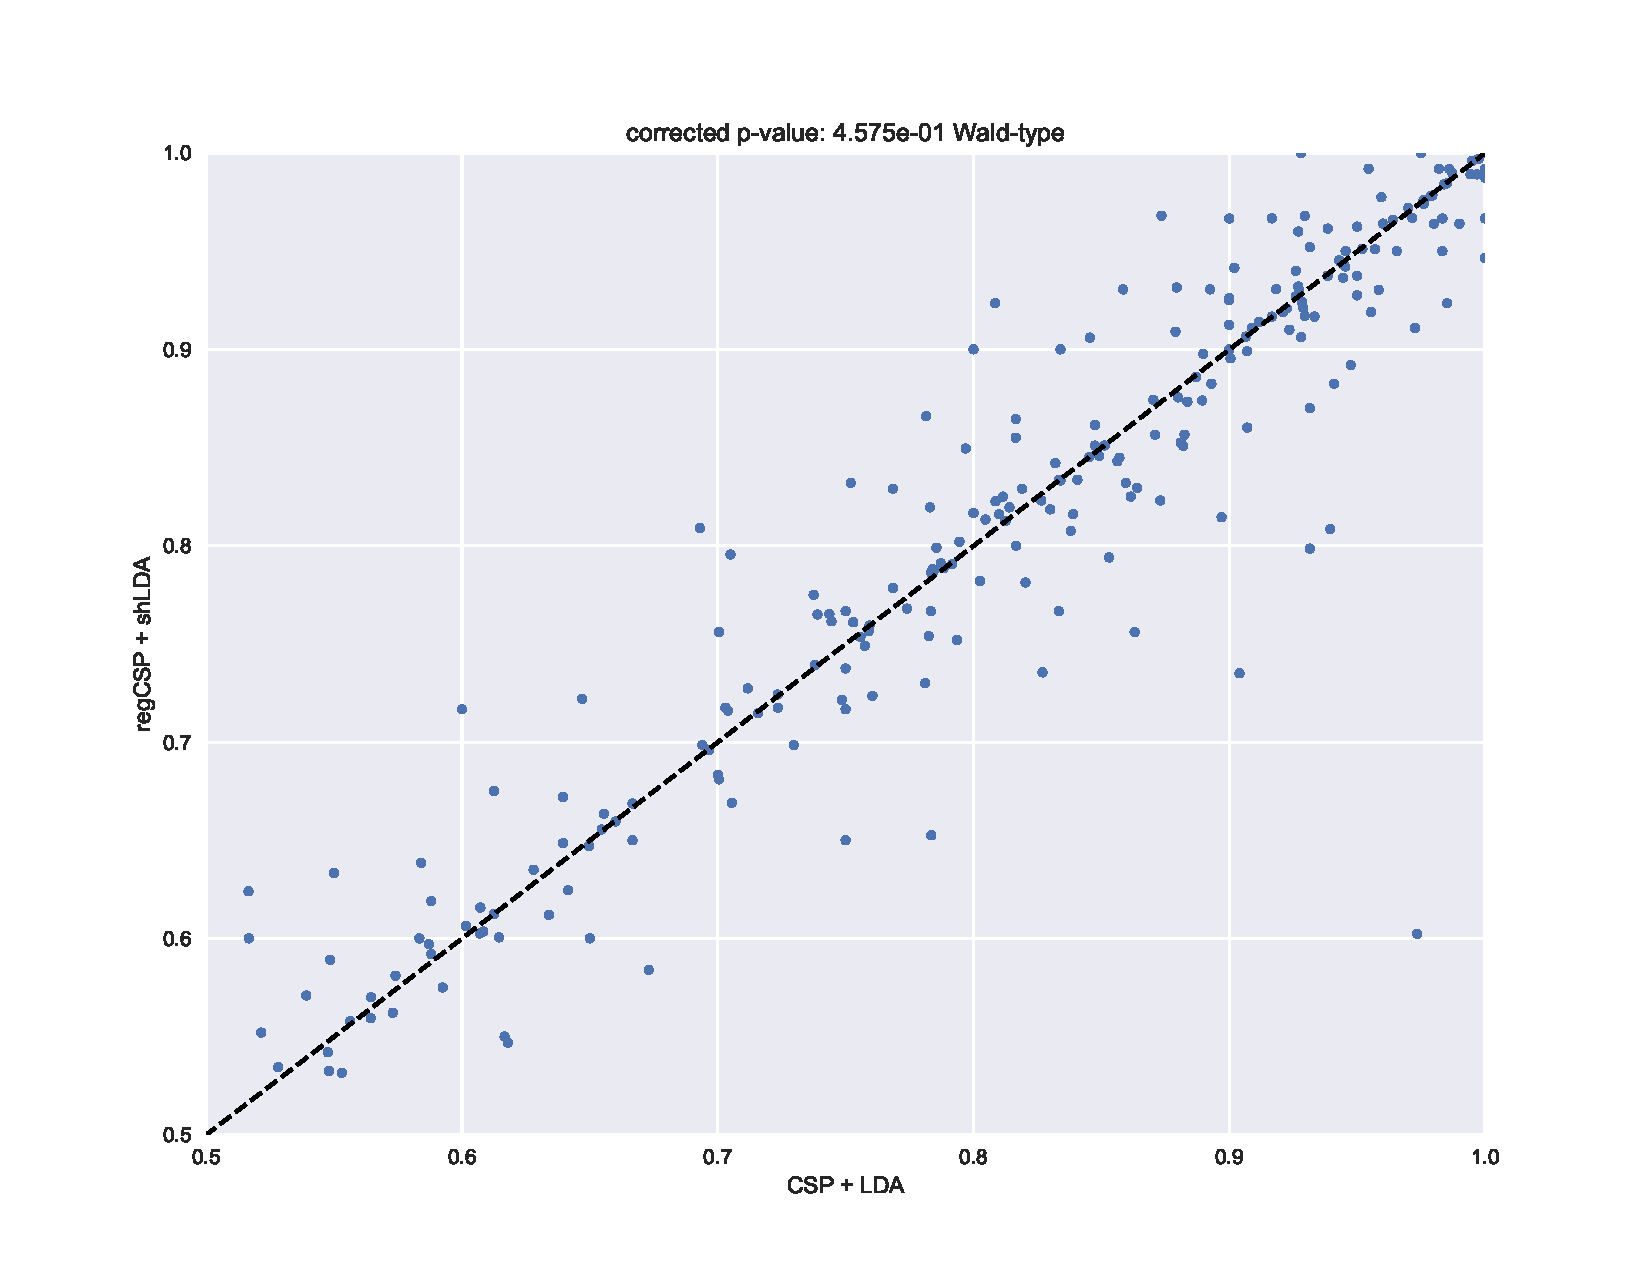
\includegraphics[width=\textwidth]{Figures/CSP1.pdf}
    \end{subfigure}%
    \begin{subfigure}{0.475\textwidth}
        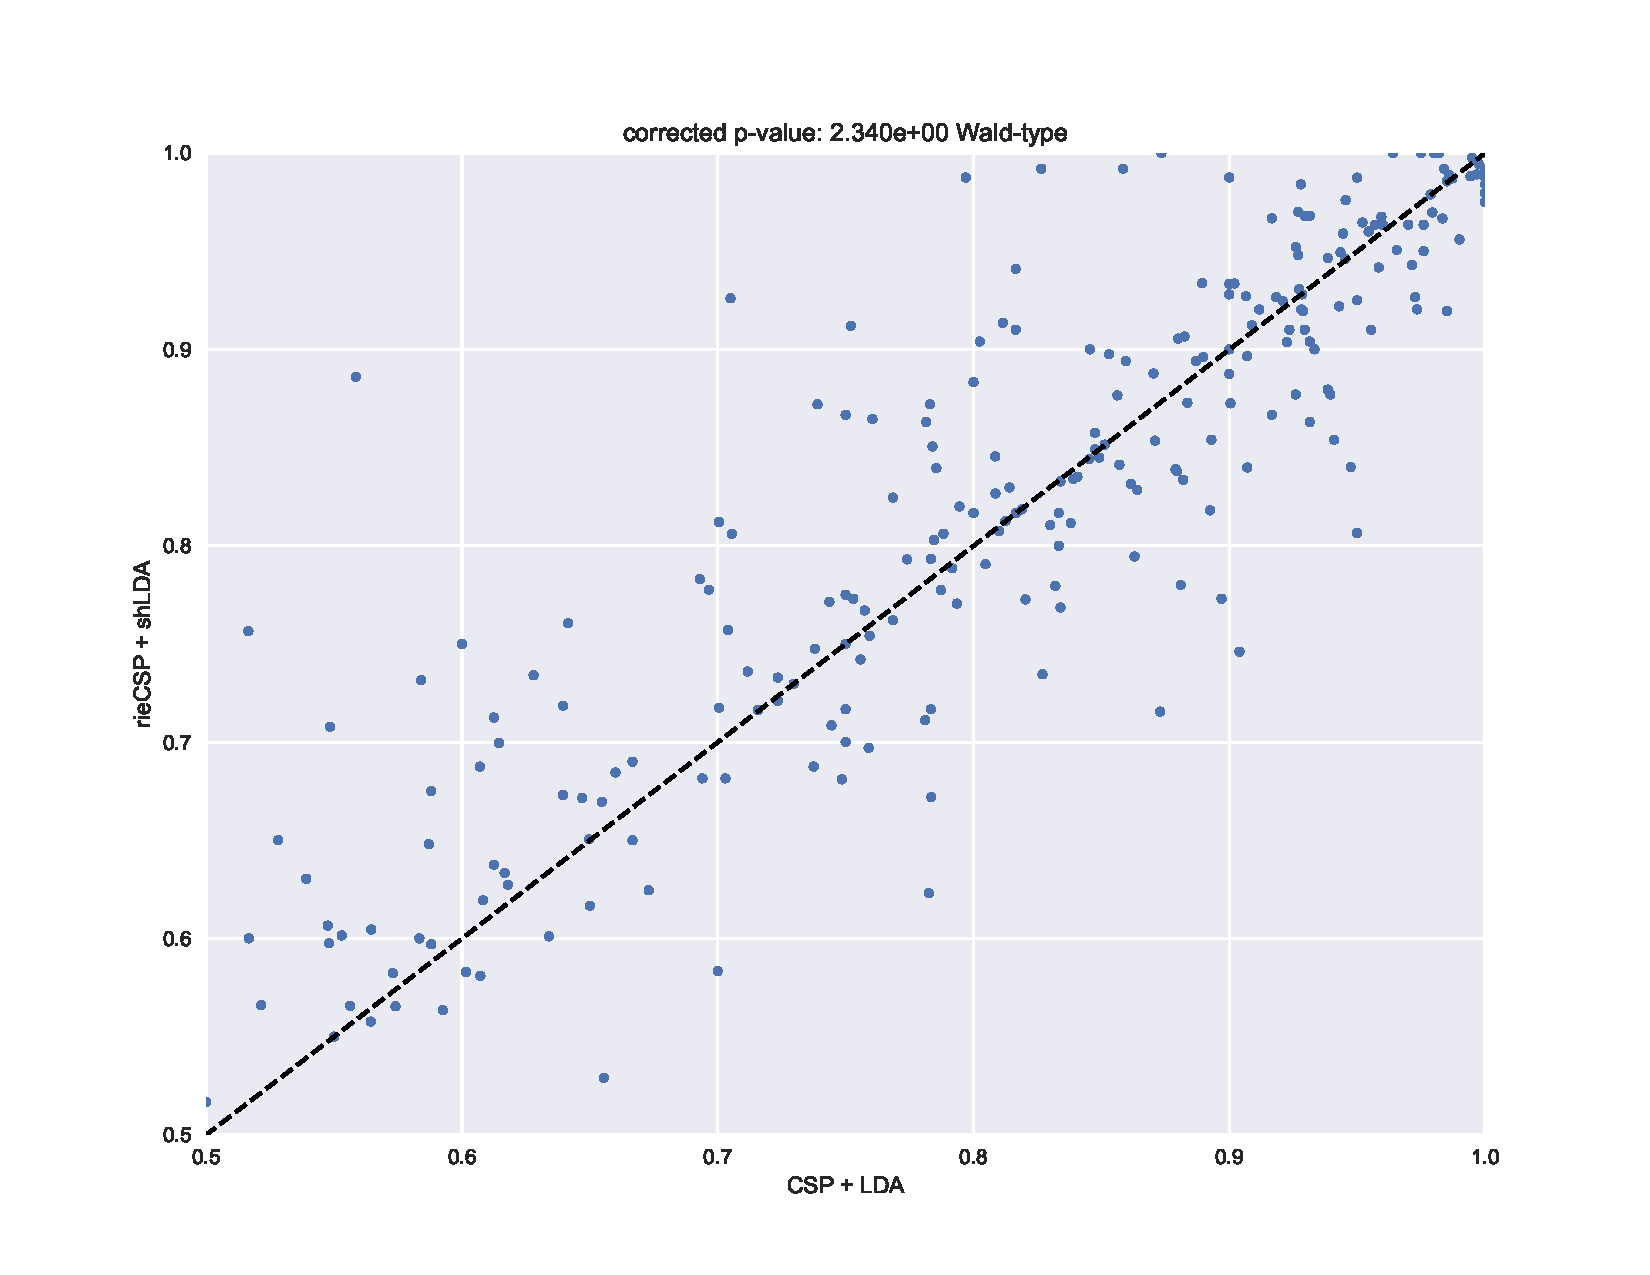
\includegraphics[width=\textwidth]{Figures/CSP2.pdf}
    \end{subfigure}
    \begin{subfigure}{0.475\textwidth}
        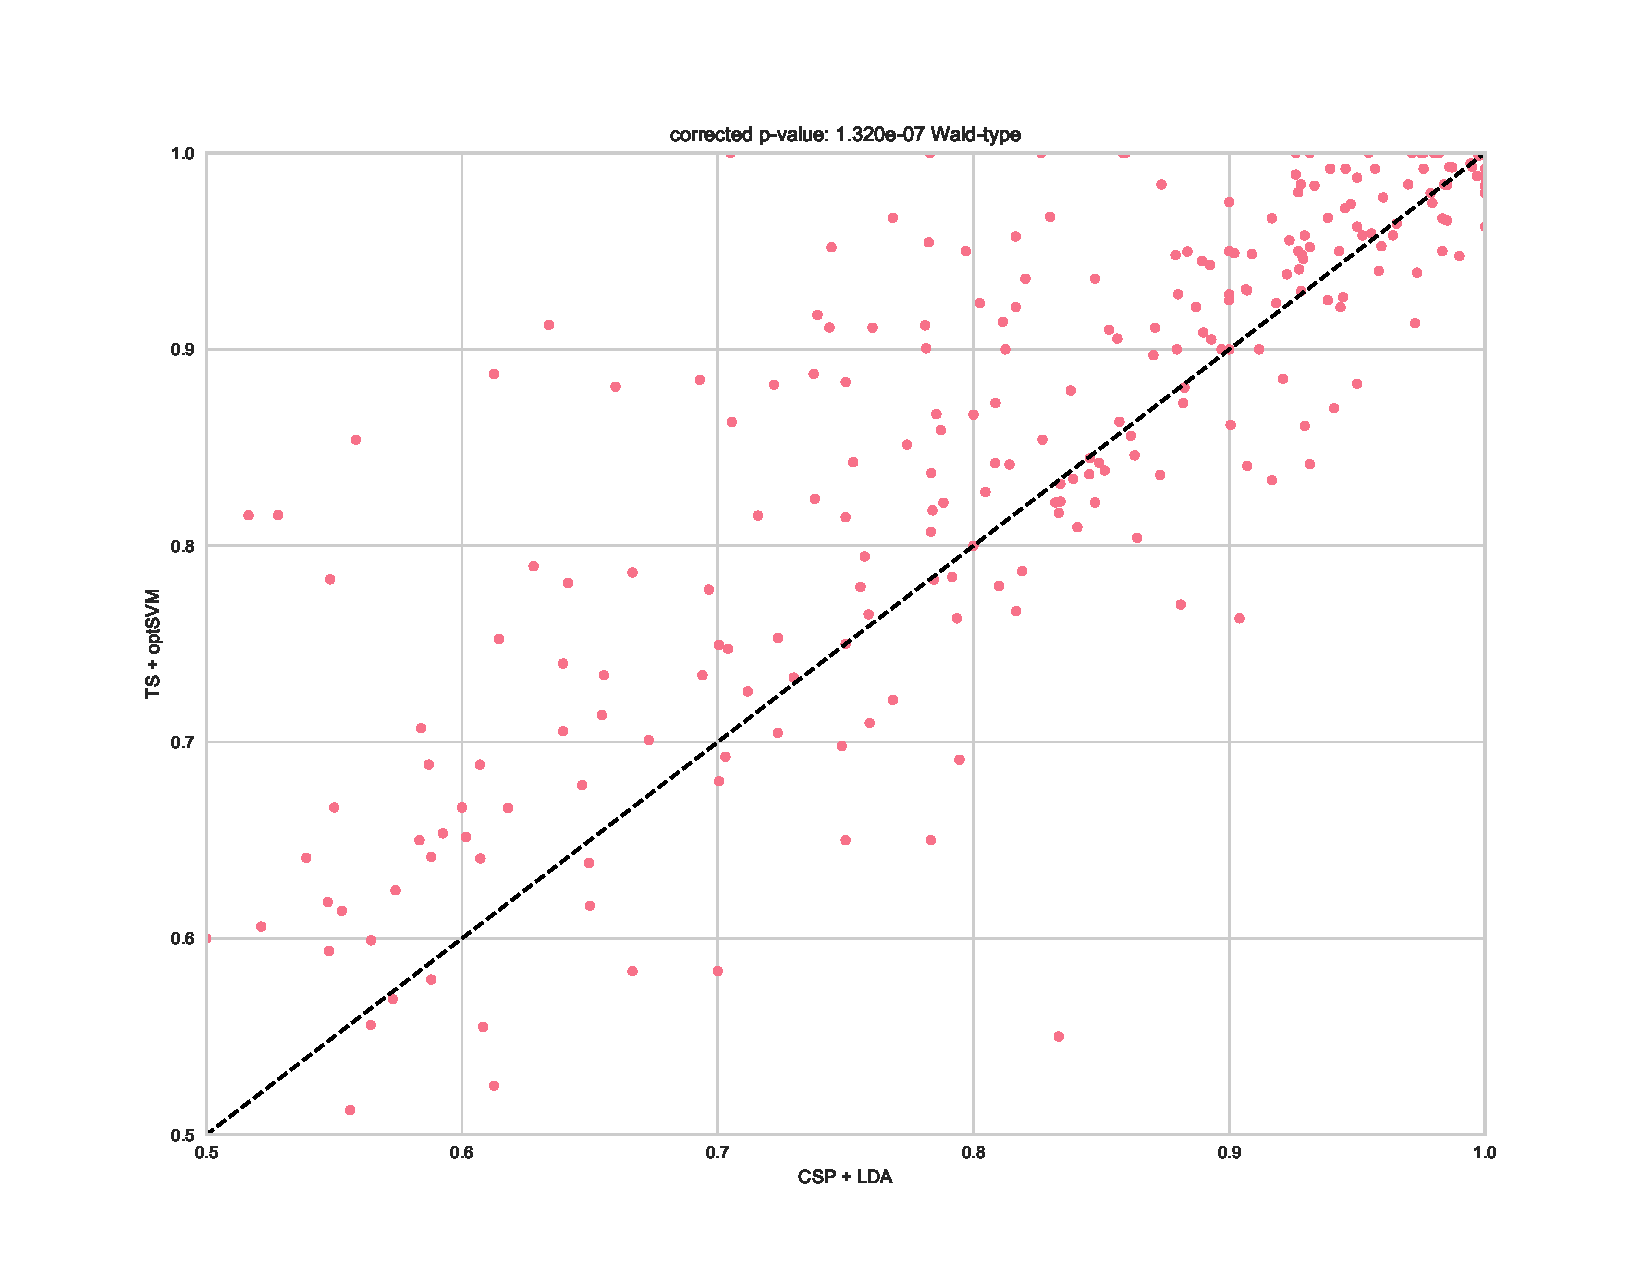
\includegraphics[width=\textwidth]{Figures/CSP3.pdf}
    \end{subfigure}
    \begin{subfigure}{0.475\textwidth}
        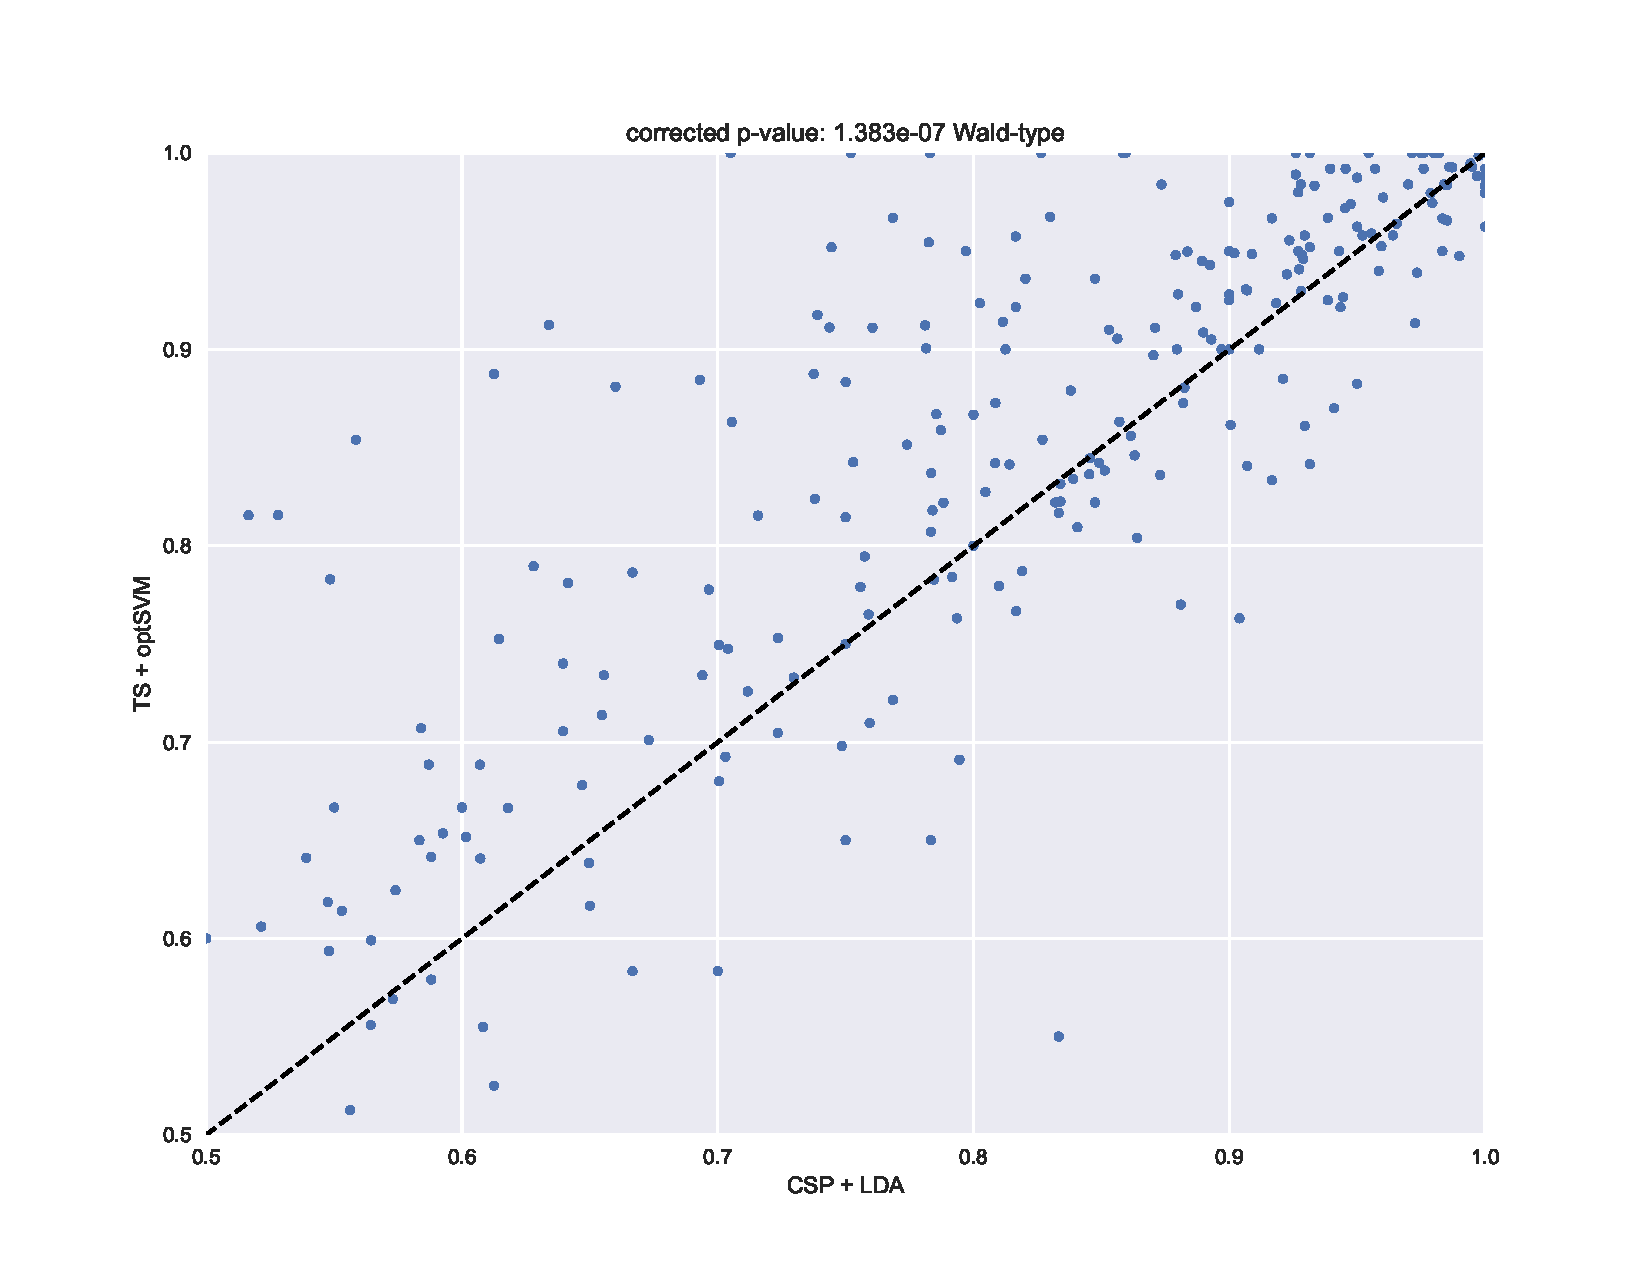
\includegraphics[width=\textwidth]{Figures/CSP4.pdf}
    \end{subfigure}
    \caption{Paired pots of CSP versus the two regularized methods, FBCSP, 
      and the tangent space SVM. Interestingly, across datasets
      neither of the regularization methods does significantly better
      in within-session classification. However, the tangent space
      method does reliably out-perform it}
    \label{fig:csp}
\end{figure*}
\begin{figure*}
  \centering
  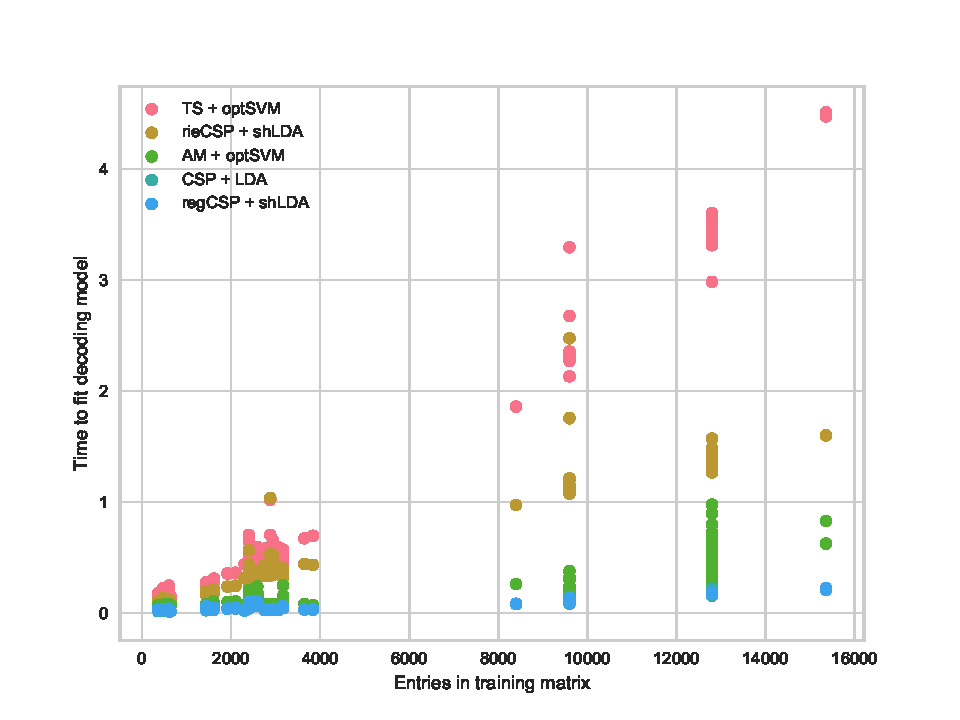
\includegraphics[width=\textwidth]{Figures/time2d.pdf}
  \caption{Time plot of all pipelines across all datasets, as a
    function of number of entries in the training matrix}
  \label{fig:time}
\end{figure*}

%%% Local Variables:
%%% mode: latex
%%% TeX-master: "main"
%%% End:
